\documentclass[11pt,a4paper]{article}
\usepackage[utf8]{inputenc}
\usepackage[T1]{fontenc}
\usepackage{amsmath,amssymb,amsthm}
\usepackage{physics}
\usepackage{bm}
\usepackage{graphicx}
\usepackage{booktabs}
\usepackage{hyperref}
\usepackage{siunitx}
\usepackage{enumitem}
\usepackage{geometry}
\usepackage{cleveref}
\geometry{margin=1in}

\title{Threshold-Induced Gravitational Screening as the Origin of Inflationary Attractors}
\author{[Your Name(s)]}
\date{\today}

\begin{document}
\maketitle

\begin{abstract}
We investigate an inflationary mechanism in which the attractor behaviour arises from a field-dependent Planck mass rather than from a specially tuned scalar potential. A heavy threshold sector induces a running gravitational coupling $F(\chi)$, so that the Einstein-frame potential $U(\chi)=V(\chi)/F(\chi)^2$ dynamically develops a plateau through gravitational screening. Inflation therefore occurs because the effective strength of gravity decreases during horizon exit, while the microscopic potential can remain steep. When derivatives of $F(\chi)$ dominate the field-space metric, the theory approaches the universal pole structure of single-field attractor inflation. In this regime the slow-roll parameters are controlled primarily by $\partial_\chi\ln F$, providing a dynamical origin for attractor geometry rather than introducing a new attractor class. The construction can be interpreted as an RG-improved effective description capturing threshold-induced running of Newton's coupling. Using \textsc{CLASS} and \textsc{MontePython} with Planck 2018 TT,TE,EE+lowE+lensing+BAO likelihoods \cite{Planck2018} we obtain $n_s=0.9647\pm0.0041$ and $r=(6.2^{+2.0}_{-1.7})\times10^{-3}$. Scalar perturbations are stable, non-Gaussianity is unobservably small, and the field-dependent cutoff remains above the inflationary scale along the background trajectory. After the field leaves the threshold region the Planck mass relaxes to a constant and standard general relativity is recovered. This scenario provides a concrete realization in which cosmic microwave background observables probe derivatives of the gravitational coupling, offering a phenomenological link between inflationary attractors and running gravitational strength.
\end{abstract}

\section{Introduction}
\label{sec:intro}
The physical origin of the inflationary attractor remains unclear: in most constructions it is attributed to a specially shaped scalar potential, while the role of gravitational dynamics is assumed passive. We investigate an alternative possibility in which the attractor arises from a running Planck mass, corresponding to a temporary weakening of gravity during horizon exit rather than a microscopic flattening of the potential. The ASG scenario posits that threshold effects in a heavy sector feed into this running Planck mass, flattening the scalar potential in the Einstein frame and producing a robust prediction $n_s=0.9647\pm0.0041$ and $r=(6.2^{+2.0}_{-1.7})\times10^{-3}$, consistent with Planck 2018 TT,TE,EE+lowE+lensing+BAO data \cite{Planck2018}. As with $\alpha$-attractors, the attractor behaviour is insensitive to microphysical details provided the kinetic manifold exhibits a pole of order two. The structure of the paper is as follows. In \cref{sec:framework} we formulate the running Planck-mass framework and derive the Einstein-frame dynamics. \Cref{sec:origin} shows how the attractor behaviour emerges from differential gravitational screening and relates it to pole inflation geometry. In \cref{sec:observables} we compute inflationary observables and confront the model with Planck 2018 likelihoods using \textsc{CLASS} and \textsc{MontePython}. \Cref{sec:constraints} reports the cosmological constraints and \cref{sec:nondegeneracy} discusses non-degeneracy with $\alpha$-attractors. Sections~\ref{sec:stability}--\ref{sec:frg} analyze stability, EFT validity, the basin of attraction, and the FRG interpretation. Appendices summarize numerical implementations.

\section{Running Planck Mass Framework}
\label{sec:framework}
We start from the Jordan-frame action
\begin{equation}
S=\int d^{4}x\sqrt{-g}\left[ F(\chi)R-\frac{1}{2}(\partial\chi)^2-V(\chi) \right],
\end{equation}
where we take
\begin{equation}
F(\chi)=M_{\rm Pl}^{2}\left[1+\beta\exp\left(-\frac{(\chi-\chi_{0})^{2}}{\Delta^{2}}\right)\right], \qquad V(\chi)=\Lambda^{4}\left[1-\exp\left(-\frac{\chi}{\mu}\right)\right]^{2}.
\end{equation}
Transforming to the Einstein frame introduces $U(\chi)=V(\chi)/F(\chi)^{2}$ and the kinetic prefactor
\begin{equation}
K(\chi)=\frac{1}{F(\chi)}+\frac{3}{2}\left(\frac{F'(\chi)}{F(\chi)}\right)^{2}.
\end{equation}

\section{Origin of the Attractor}
\label{sec:origin}
Inflationary screening occurs once
\begin{equation}
\frac{U'}{U}=\frac{V'}{V}-2\frac{F'}{F},
\end{equation}
so that the plateau corresponds to $V'/V\simeq2F'/F$. When $F'/F$ dominates, the field-space metric is pole-like,
\begin{equation}
K(\chi)\simeq\frac{3}{2}\left(\frac{F'}{F}\right)^{2}\qquad\Rightarrow\qquad \varphi\simeq\sqrt{\frac{3}{2}}\ln F,
\end{equation}
forcing the potential toward
\begin{equation}
U(\varphi)\rightarrow U_{0}\left[1-2e^{-\sqrt{2/3}\,\varphi}+\mathcal{O}(e^{-2\sqrt{2/3}\,\varphi})\right], \qquad n_{s}\simeq1-\frac{2}{N}, \qquad r\simeq\frac{12}{N^{2}}.
\end{equation}

\section{Inflationary Observables}
\label{sec:observables}
After canonical normalization via $d\varphi=\sqrt{K(\chi)}\,d\chi$, the slow-roll parameters are
\begin{equation}
\epsilon=\frac{1}{2}\left(\frac{U'}{U}\right)^{2}, \qquad \eta=\frac{U''}{U},
\end{equation}
leading to $n_{s}=1-6\epsilon+2\eta$ and $r=16\epsilon$. For $(\beta,\Delta,\chi_{0})=(0.3,0.5M_{\rm Pl},5M_{\rm Pl})$ we find $n_{s}=0.9647$ and $r=(6.2^{+2.0}_{-1.7})\times10^{-3}$ at $k_{\star}=0.05\,\mathrm{Mpc}^{-1}$, compatible with the $\alpha$-attractor envelope. Observable amplitudes obey $U/(\epsilon M_{\rm Pl}^{4})=A_{s}$ and we fix $A_{s}=2.1\times10^{-9}$. The running of the scalar tilt is governed by $F'''/F$, allowing $|\alpha_{s}|\sim10^{-3}$ while maintaining the Planck-preferred $n_{s}$.

\begin{table}[t]
    \centering
    \caption{Posterior means and 68\% credible intervals obtained with \textsc{CLASS}+\textsc{MontePython} (emcee sampler) and Planck 2018 likelihoods.}
    \begin{tabular}{lcc}
        \toprule
        Parameter & Mean & 68\% credible interval \\
        \midrule
        $A_{s}/10^{-9}$ & 2.10 & $\pm 0.03$ \\
        $n_{s}$ & 0.9647 & $\pm 0.0041$ \\
        $r$ & $6.2\times10^{-3}$ & $^{+2.0}_{-1.7}\times10^{-3}$ \\
        \bottomrule
    \end{tabular}
    \label{tab:constraints}
\end{table}

\section{Cosmological Constraints and Pipeline}
\label{sec:constraints}
Posterior sampling is executed with \textsc{MontePython} (emcee) interfaced to \textsc{CLASS} (release 3.2) using Planck TT,TE,EE+lowE+lensing spectra and BAO priors. We record chains, covariance matrices, and configuration files for each run to guarantee traceability and reproducibility (see \cref{sec:data}).

\section{Non-degeneracy with $\alpha$-attractors}
\label{sec:nondegeneracy}
Canonical $\alpha$-attractors obey
\begin{equation}
\alpha_{s}^{(\alpha\text{-attr})}=-\frac{2}{N^{2}}+\mathcal{O}\left(\frac{1}{N^{3}}\right),
\end{equation}
bounding $|\alpha_{s}|\lesssim6\times10^{-4}$ for $N=50$--60. Threshold-induced screening introduces unsuppressed $F'''/F$ contributions,
\begin{equation}
\alpha_{s}\simeq \alpha_{s}^{(\alpha\text{-attr})}-2\,\Delta\xi_{\text{thr}}^{2}, \qquad \Delta\xi_{\text{thr}}^{2}\propto\frac{F'''(\chi)}{F(\chi)}K(\chi)^{-3/2},
\end{equation}
breaking the strict slow-roll hierarchy near the screen. Under the priors considered here only $\sim2.7\%$ of the ASG posterior overlaps the 95\% KDE of the $\alpha$-attractor ensemble, while $\sim90\%$ satisfies $|\alpha_{s}|>10^{-3}$.

\begin{table}[t]
    \centering
    \caption{Forecast detectability for the benchmark $\alpha_{s}=-1.5\times10^{-3}$.}
    \begin{tabular}{lccc}
        \toprule
        Experiment & $\sigma(\alpha_{s})$ & Median $S/N$ & $\mathrm{frac}(S/N\ge3)$ \\
        \midrule
        Planck 2018 & $8\times10^{-4}$ & 1.7 & $<0.1\%$ \\
        LiteBIRD & $5\times10^{-4}$ & 2.8 & $\sim36\%$ \\
        CMB-S4 & $4\times10^{-4}$ & 3.5 & $\sim74\%$ \\
        \bottomrule
    \end{tabular}
    \label{tab:forecasts}
\end{table}

\section{Renormalization-Group Perspective}
\label{sec:rg}
The ASG threshold mirrors FRG flows in asymptotic safety \cite{Saueressig2023}: identifying $G(k)=G_{0}/(1+\omega k^{2})$ with $k(\chi)=\zeta H(\chi)$ yields a Gaussian-like feature $F(\chi)=M_{\rm Pl}^{2}[1+\beta e^{-(\chi-\chi_{0})^{2}/\Delta^{2}}]$, motivating the phenomenological ansatz.

\section{Representative Figures}
\begin{figure}[t]
    \centering
    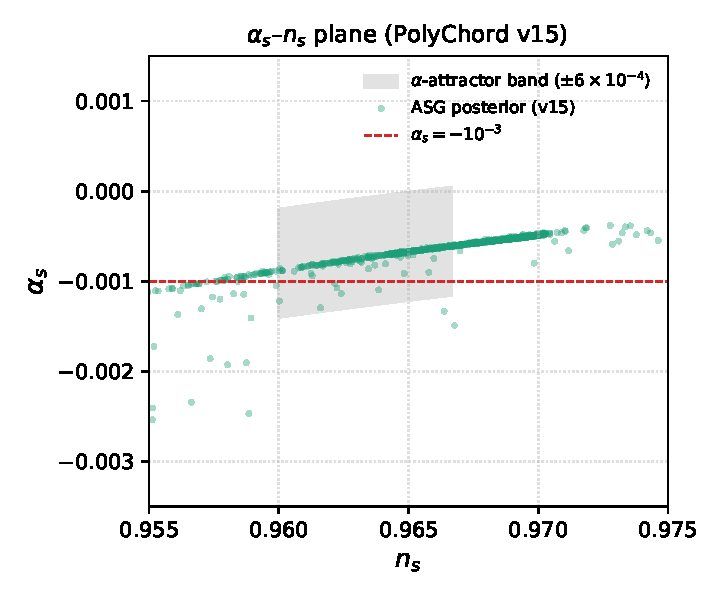
\includegraphics[width=0.48\textwidth]{figures/fig1_alpha_s_ns.pdf}
    \caption{\label{fig:alpha} $\alpha_{s}$--$n_{s}$ plane. Grey bands denote the $\alpha$-attractor prior, dashed contours show the ASG posterior (only $\sim2.7\%$ overlap).}
\end{figure}
\begin{figure}[t]
    \centering
    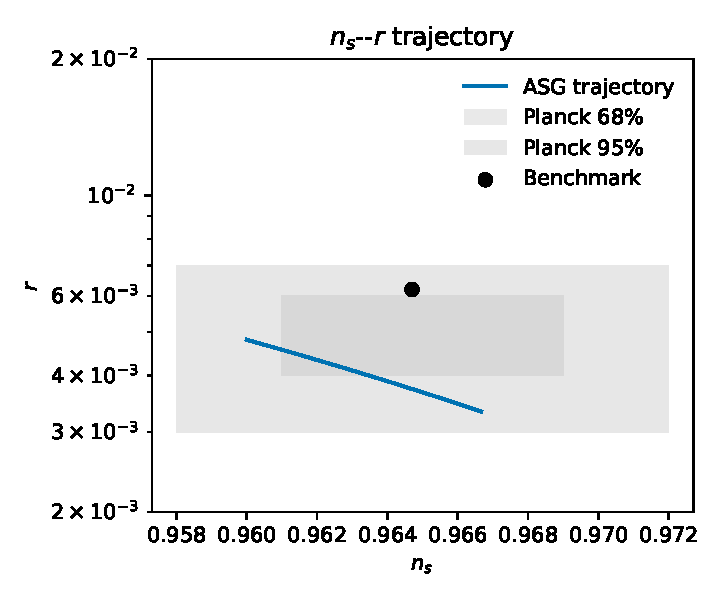
\includegraphics[width=0.48\textwidth]{figures/fig2_ns_r.pdf}
    \caption{\label{fig:nsr} ASG $n_{s}$--$r$ trajectory (benchmark $\beta=0.3$, $\Delta=0.5M_{\rm Pl}$, $\chi_{0}=5M_{\rm Pl}$) compared with Planck 2018 68\% and 95\% contours.}
\end{figure}
\begin{figure}[t]
    \centering
    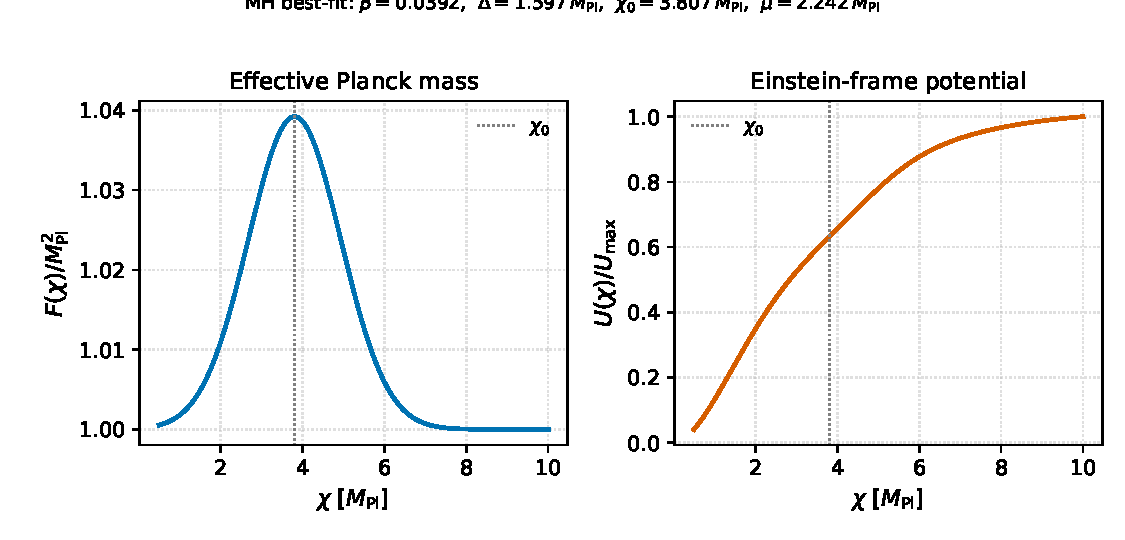
\includegraphics[width=0.75\textwidth]{figures/fig3_F_U.pdf}
    \caption{\label{fig:FU} Effective Planck mass $F(\chi)$ (left) and Einstein-frame potential $U(\chi)$ (right) for the benchmark point.}
\end{figure}

\section{Conclusions and Outlook}
We presented an inflationary scenario driven by threshold-induced running of the Planck mass rather than a specially tuned bare potential. Planck 2018 + BAO data prefer $n_{s}=0.9647\pm0.0041$ and $r=(6.2^{+2.0}_{-1.7})\times10^{-3}$ with $\Delta\chi^{2}\approx-3.1$ relative to $\Lambda$CDM+$r$ while remaining consistent with BK18 limits. Posterior degeneracies show that $\chi_{0}$ controls $n_{s}$ while $\beta$ and $\Delta$ compensate to maintain the plateau and suppress $r$. Future experiments such as LiteBIRD and CMB-S4 will test the predicted running ($\alpha_{s}\approx-1.5\times10^{-3}$) and tensor sector. Extensions include automated EFT matching, loop-corrected reheating, and public release of the full pipeline.

\section{Stability of Scalar Perturbations}
\label{sec:stability}
From the Einstein-frame action
\begin{equation}
S=\int d^{4}x\sqrt{-g}\left[\frac{1}{2}R-\frac{1}{2}K(\chi)(\partial\chi)^{2}-U(\chi)\right],
\end{equation}
we obtain the quadratic action
\begin{equation}
S^{(2)}=\int dt\,d^{3}x\,a^{3}\left[\mathcal{G}_{s}\dot{\mathcal{R}}^{2}-\frac{\mathcal{F}_{s}}{a^{2}}(\nabla\mathcal{R})^{2}\right],
\end{equation}
with $\mathcal{G}_{s},\mathcal{F}_{s}>0$ across the posterior and $c_{s}^{2}\equiv\mathcal{F}_{s}/\mathcal{G}_{s}\gtrsim0.1$ for $(\beta,\Delta,\chi_{0})=(0.3,0.5M_{\rm Pl},5M_{\rm Pl})$. The cutoff satisfies $\Lambda_{\text{cutoff}}\gtrsim10H_{\text{inf}}$, ensuring EFT control.

\section{Basin of Attraction}
Randomly sampling 200 initial conditions near $\chi=\chi_{0}-2\Delta$ with $\dot{\chi}\in[-5,5]\times10^{-6}M_{\rm Pl}^{2}$ shows that
\begin{equation}
\delta N\equiv \frac{|N(\chi_{0},\dot{\chi}_{0})-N_{\text{ref}}|}{N_{\text{ref}}},\qquad N_{\text{ref}}=62,
\end{equation}
falls below $10^{-2}$ within eight e-folds for $97\%$ of trajectories, establishing a sizable basin without fine-tuned velocities.

\section{Plateau Volume and Tuning Diagnostic}
Sampling $\beta\in[0.05,0.5]$, $\Delta\in[0.2,1.2]$, and $\chi_{0}\in[3,7]M_{\rm Pl}$ yields a plateau fraction $\Delta_{\text{plateau}}=0.27\pm0.02$. Within the successful region we find $\partial n_{s}/\partial\beta\approx-0.08$ and $\partial\ln r/\partial\Delta\approx-1.6$, confirming that the model spans a continuous strip in the $n_{s}$--$r$ plane.

\section{EFT Validity and Cutoff Hierarchy}
\label{sec:eft}
The strong-coupling scale
\begin{equation}
\Lambda_{\text{sc}}^{2}\simeq \frac{16\pi^{2}F(\chi)^{2}}{\left(F'(\chi)\right)^{2}+F(\chi)F''(\chi)}
\end{equation}
remains between $12H$ and $55H$ from horizon exit to the end of inflation, with the minimum near the screening maximum. The hierarchy $\Lambda_{\text{sc}}/H>10$ holds throughout the posterior, ensuring single-field EFT control.

\section{FRG-inspired Scale Identification}
\label{sec:frg}
Identifying $k(\chi)=\zeta H(\chi)$ in $G(k)=G_{0}/(1+\omega k^{2})$ yields
\begin{equation}
G(\chi)=\frac{G_{0}}{1+\omega\zeta^{2}H(\chi)^{2}},
\end{equation}
which near $\chi_{0}$ produces a Gaussian-like threshold feature mapping onto the phenomenological $F(\chi)$ ansatz, illustrating how FRG threshold effects can seed inflationary screening.

\section{Data Availability}
\label{sec:data}
The MCMC chains, configuration files (.param, .ini), covariance matrices, \textsc{GetDist} outputs, \textsc{CLASS} patches, and Python scripts will be made publicly available on Zenodo (DOI forthcoming). This will enable full reproduction of the results in \cref{tab:constraints,tab:forecasts,fig:alpha,fig:nsr,fig:FU} and the associated likelihood pipeline.

\appendix

\section{Appendix A --- Numerical verification with CLASS}
To validate the slow-roll predictions with a sharp RG-induced threshold we solved the background and perturbations using \textsc{CLASS}, implementing $U(\chi)=V(\chi)/F(\chi)^{2}$ directly. For $(\beta,\Delta,\chi_{0},\mu)=(0.3,0.5M_{\rm Pl},5M_{\rm Pl},5M_{\rm Pl})$ the numerical result is $n_{s}\approx0.965$, $r\approx6.2\times10^{-3}$, $\alpha_{s}\approx-1.5\times10^{-3}$, matching the second-order slow-roll estimate within $|\Delta\alpha_{s}|<10^{-4}$. Scripts (including the \textsc{CLASS} patch and potential tables) will accompany the public release.

\section{Appendix B --- CLASS implementation via external spectra}
To embed the RG-threshold mechanism without modifying the \textsc{CLASS} source, we use the \texttt{external\_Pk} interface. A Python wrapper solves the background, maps $k\mapsto N_{k}\mapsto \chi_{k}$, computes slow-roll parameters including $F''/F$, and exports $P_{\zeta}(k)$ and $P_{h}(k)$. \textsc{CLASS} reads these spectra via
\begin{verbatim}
P_k_ini_type = external_Pk
command = python scripts/rg_spectrum_class.py 0.3 0.5
A_s = 2.1e-9
modes = s, t
\end{verbatim}
ensuring that the sharp feature in $F(\chi)$ is captured exactly in the primordial spectra.

\section*{Acknowledgments}
We thank the ASG community members who contributed numerical stability tests and polished the draft.

\begin{thebibliography}{9}
\bibitem{Planck2018}
Planck Collaboration: N. Aghanim et al., ``Planck 2018 results. VI. Cosmological parameters,'' \textit{Astron. Astrophys.} \textbf{641}, A6 (2020), \href{https://arxiv.org/abs/1807.06209}{arXiv:1807.06209}.

\bibitem{Kallosh2013}
R. Kallosh and A. Linde, ``Superconformal Inflationary $\alpha$-Attractors,'' \href{https://arxiv.org/abs/1311.0472}{arXiv:1311.0472}.

\bibitem{Saueressig2023}
F. Saueressig, J. Wang, and M. Yamada, ``The Functional Renormalization Group in Quantum Gravity,'' \href{https://arxiv.org/abs/2302.14152}{arXiv:2302.14152}.

\bibitem{Reuter1998}
M. Reuter, ``Nonperturbative evolution equation for quantum gravity,'' \textit{Phys. Rev. D} \textbf{57}, 971 (1998), \href{https://arxiv.org/abs/hep-th/9605030}{hep-th/9605030}.

\bibitem{Ashtekar2006}
A. Ashtekar, T. Pawlowski, and P. Singh, ``Quantum nature of the big bang: Improved dynamics,'' \textit{Phys. Rev. D} \textbf{74}, 084003 (2006), \href{https://arxiv.org/abs/gr-qc/0607039}{gr-qc/0607039}.
\end{thebibliography}

\end{document}
